\apendice{Especificación de diseño}

\section{Introducción}
En esta sección se va a hablar de los aspectos más relevantes del diseño de la aplicación de Android.
\begin{itemize}
	\item En primer lugar, se hará una breve mención al diseño de los datos.
	\item A continuación, en el apartado de diseño procedimental se expondrán detalladamente los dos procesos más relevantes de la aplicación, y en los que se basa fundamentalmente su comportamiento, obviando otros procesos más sencillos o basados en objetos propios del \textit{framework} de Android cuyo funcionamiento puede encontrarse en la documentación.
	\item Después se expondrán las características de la arquitectura general de la aplicación, considerando dos puntos de vista que pueden servir para definir de forma complementaria la arquitectura general del sistema. 
	\item Por último se expondrán los prototipos de la interfaz de usuario generados antes del desarrollo de la aplicación. 
\end{itemize}

\section{Diseño de datos}

Para el desarrollo de la aplicación Android no podemos hablar estrictamente de un diseño de los datos, ya que se trata de un cliente que no interactúa directamente con la base de datos. El acceso a la persistencia se hace a través de peticiones a la API del servidor, la cual devuelve siempre todos los datos en un objeto con formato JSON. 

En este sentido, podemos abstraernos del diseño e implementación concretos de la base de datos, ya que nuestra gestión de los datos solo depende de las características del JSON que nos va a devolver cada petición. La estructura de la respuesta de cada petición a la API se especifica en el Manual del programador de mi compañero José Luis Garrido Labrador. 

\section{Diseño procedimental}

Como se explica más adelante, el funcionamiento general de la aplicación se basa en la comunicación con la API del servidor remoto, el cual proporciona el modelo de datos y la lógica de negocio. Por esta razón, los procesos más relevantes corresponden con los que permiten realizar la comunicación de la aplicación con la API del servidor remoto. 

Tal y como se ha planteado la aplicación de Android, existen dos procesos relevantes que es importante entender, ya que supondrán la base del funcionamiento de la aplicación:

\begin{itemize}
	\item En primer lugar, la \textbf{llamada a los servicios genéricos de la API}. Todas las interacciones con la lógica de negocio de la aplicación (iniciar sesión, visualizar usuarios, añadir usuarios...) se realizan de esta manera. Por esta razón, para garantizar el buen funcionamiento de la aplicación, este proceso debe incluir una comprobación sobre si existe conexión a internet, si la sesión está activa y si la respuesta de la API es la esperada.
	
	Esta interacción se representa en el diagrama de secuencias de la figura~\ref{fig:sequenceAPI}. El elemento \textit{Activity} corresponde con cualquiera de las clases que extienden de \textit{AppCompatActivity} desde las que se realiza una petición a la API del servidor. 
	
	\item En segundo lugar, \textbf{la petición y recepción de los datos de una cama en tiempo real}. Este proceso se realiza a través de conexión a nivel de \textit{sockets} con el servidor y la gestión de eventos empleando la librería Socket.IO. 
	
	Esta interacción se representa en el diagrama de secuencias de la figura~\ref{fig:sequenceStreaming}. Los mensajes \texttt{give\_me\_data} y \texttt{package} son eventos de Socket.IO definidos por el programador de la API. 
\end{itemize}

\begin{figure}[H]
	\centering
	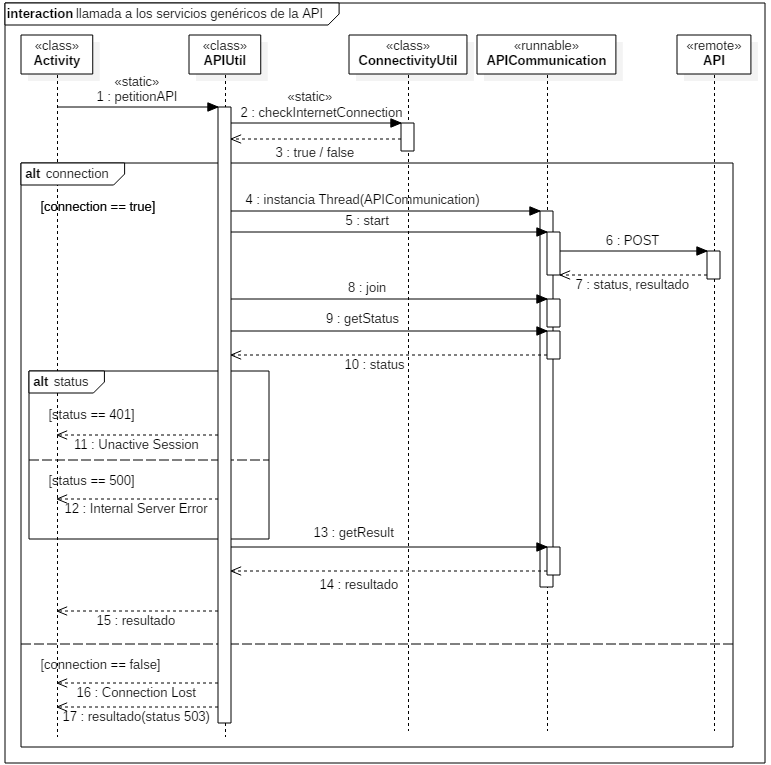
\includegraphics[width=1\textwidth]{../img/sequenceAPI.png}
	\caption{Diagrama de secuencias, llamada a los servicios genéricos de la API.}
	\label{fig:sequenceAPI}
\end{figure}

\begin{figure}[H]
	\centering
	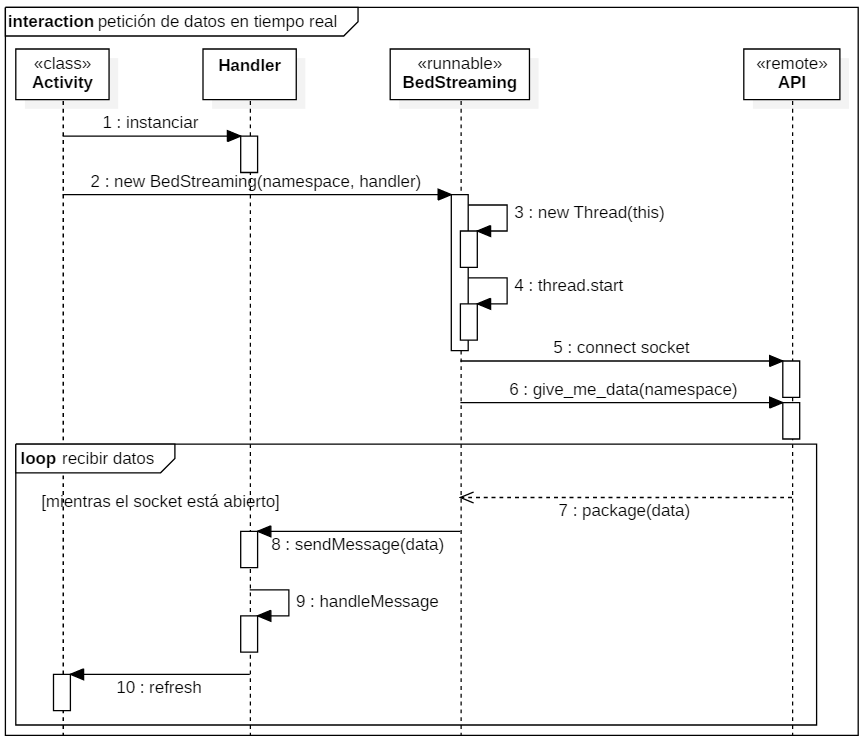
\includegraphics[width=1\textwidth]{../img/sequenceStreaming.png}
	\caption{Diagrama de secuencias, petición de datos en tiempo real.}
	\label{fig:sequenceStreaming}
\end{figure}

El funcionamiento del resto de procesos es fácilmente deducible a partir del código o corresponde con el uso de elementos propios del \textit{framework} de Android. La especificación y funcionamiento de estos elementos se puede consultar en la página web oficial de \textit{Android Developers}~\cite{androiddevelopers}.  

\section{Diseño arquitectónico}

La arquitectura de la aplicación puede verse desde varios puntos de vista. En el contexto del patrón arquitectónico Modelo-Vista-Controlador (MVC)~\cite{wiki:mvc} definimos tres componentes: 
\begin{itemize}
	\item \textbf{Modelo:} Contiene la estructura de los datos que maneja el programa e interactúa con la persistencia para realizar consultas y actualizaciones. 
	\item \textbf{Vista:} Presenta los datos del modelo y la interacción con la lógica de negocio de forma adecuada para el usuario. 
	\item \textbf{Controlador:} Responde a eventos generados por la interacción del usuario con la vista y realiza peticiones de consulta/actualización al modelo. Se puede ver como un intermediario entre ambos componentes. 
\end{itemize}

Según la definición de los componentes de este patrón, la aplicación Android podría ser considerada únicamente como un componente <<Vista>> de un sistema más grande formado también por los los servicios proporcionados por la API del servidor remoto, la cual proporciona el acceso a la persistencia y la comunicación entre el modelo de datos y la aplicación. 

Por otro lado, cuando se habla de este tipo de aplicaciones, es común encontrarnos con el término \textbf{<<arquitectura de microservicios>>}. Según esta arquitectura, cada funcionalidad se encuentra contenida en un proceso del servidor al que llamaremos microservicio. Cada microservicio encapsula un solo aspecto de la lógica de negocio, y los microservicios son procesos independientes entre sí. Tal y como ocurre en esta aplicación Android, el cliente se limita a hacer peticiones a los microservicios de la API del servidor remoto, los cuales, basándose en la lógica de negocio, le proporcionan los datos necesarios para actualizar la <<vista>> o interfaz de usuario. 

\begin{figure}[H]
	\centering
	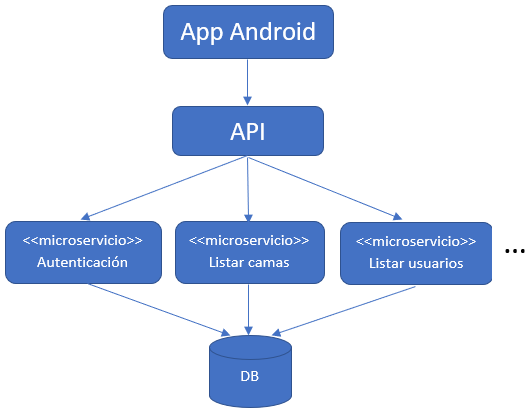
\includegraphics[width=0.8\textwidth]{../img/microservicios.png}
	\caption{Abstracción de la arquitectura de microservicios.}
	\label{fig:microservicios}
\end{figure}

\section{Diseño de interfaces}

Inicialmente se realizaron una serie de prototipos básicos en los que se plasmaron las principales funcionalidades de la aplicación, sin prestar especial atención a los aspectos estéticos de la misma. Para ello se usó la herramienta de prototipado Pencil, ya que permite incorporar elementos propios de la guía de estilos que se ha seguido para el diseño de las interfaces de usuario: \textit{Material Design}. 

\begin{figure}[H]
	\centering
	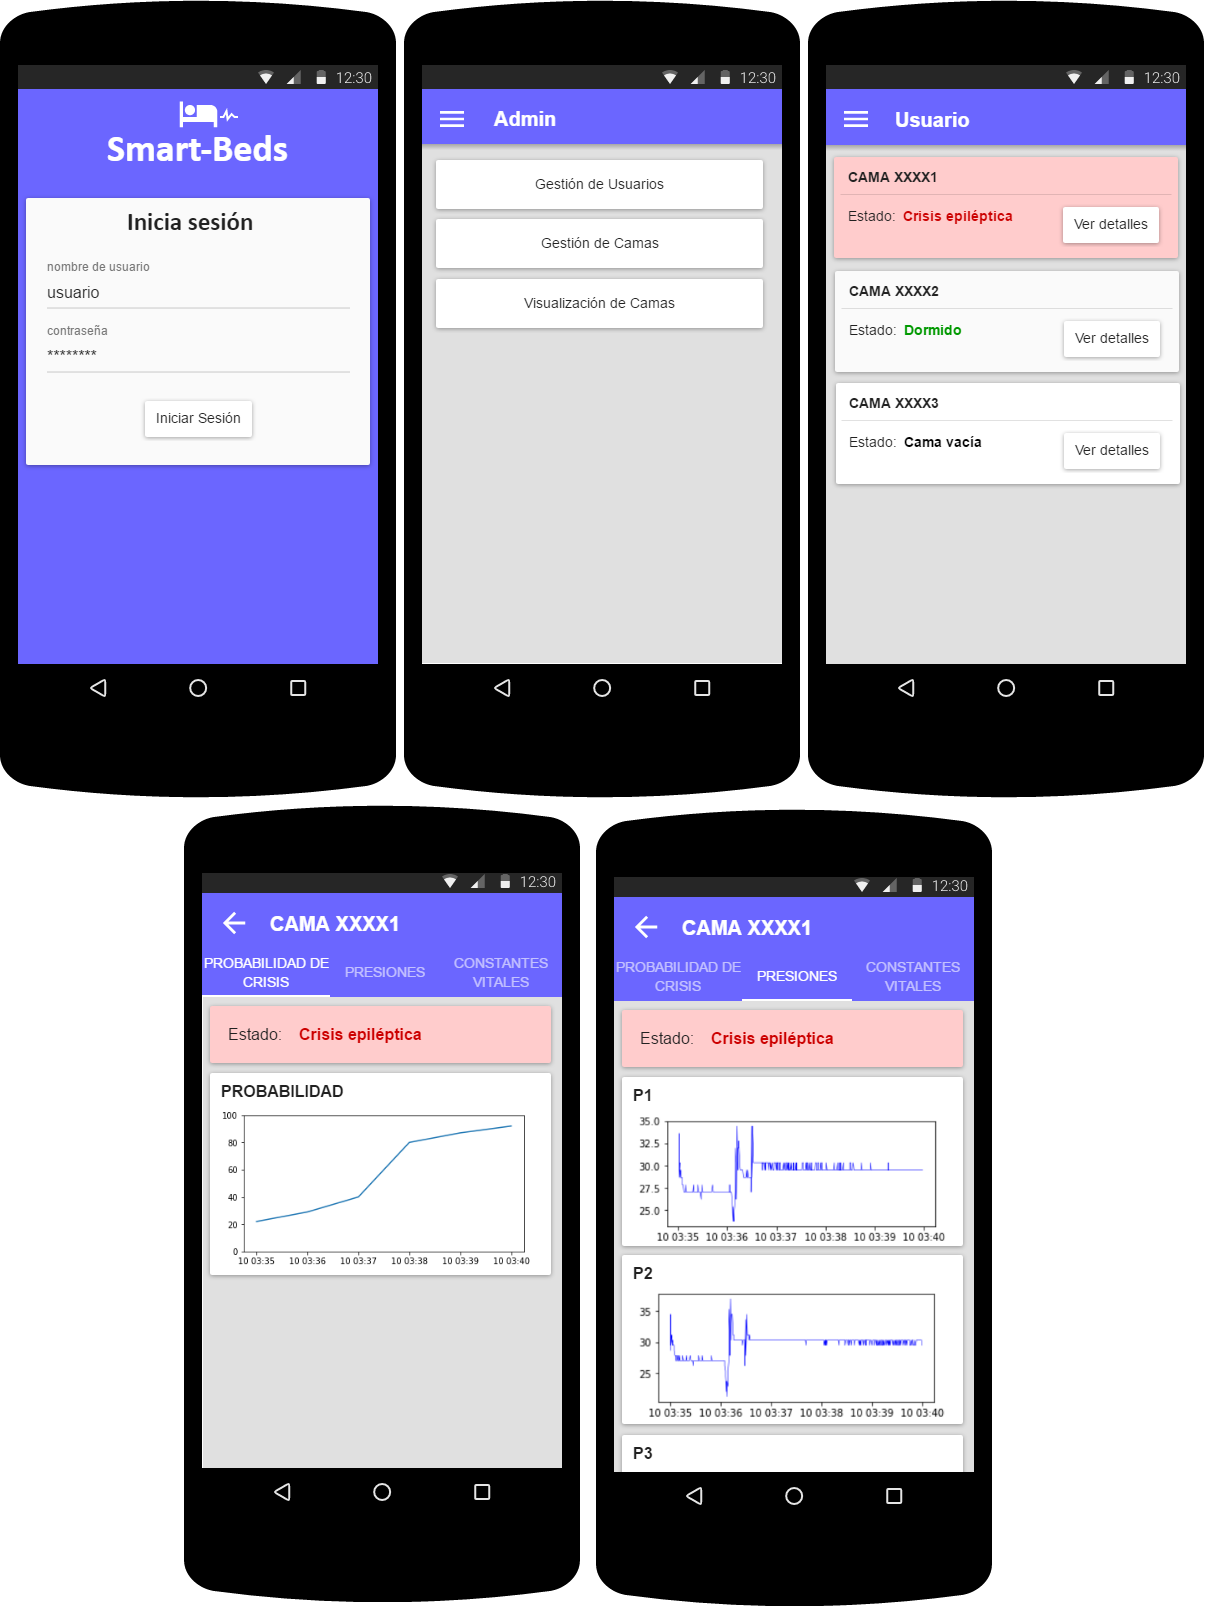
\includegraphics[width=0.75\textwidth]{../img/prototipos.png}
	\caption{Prototipos iniciales de las pantallas de: login, administración, visualización de camas y visualización de datos.}
	\label{fig:prototipos}
\end{figure}

Durante el proceso de desarrollo se tomaron varias decisiones de diseño cuyo resultado fueron las interfaces de usuario finales que se muestran en la figura~\ref{fig:interfaces}

\begin{figure}[H]
	\centering
	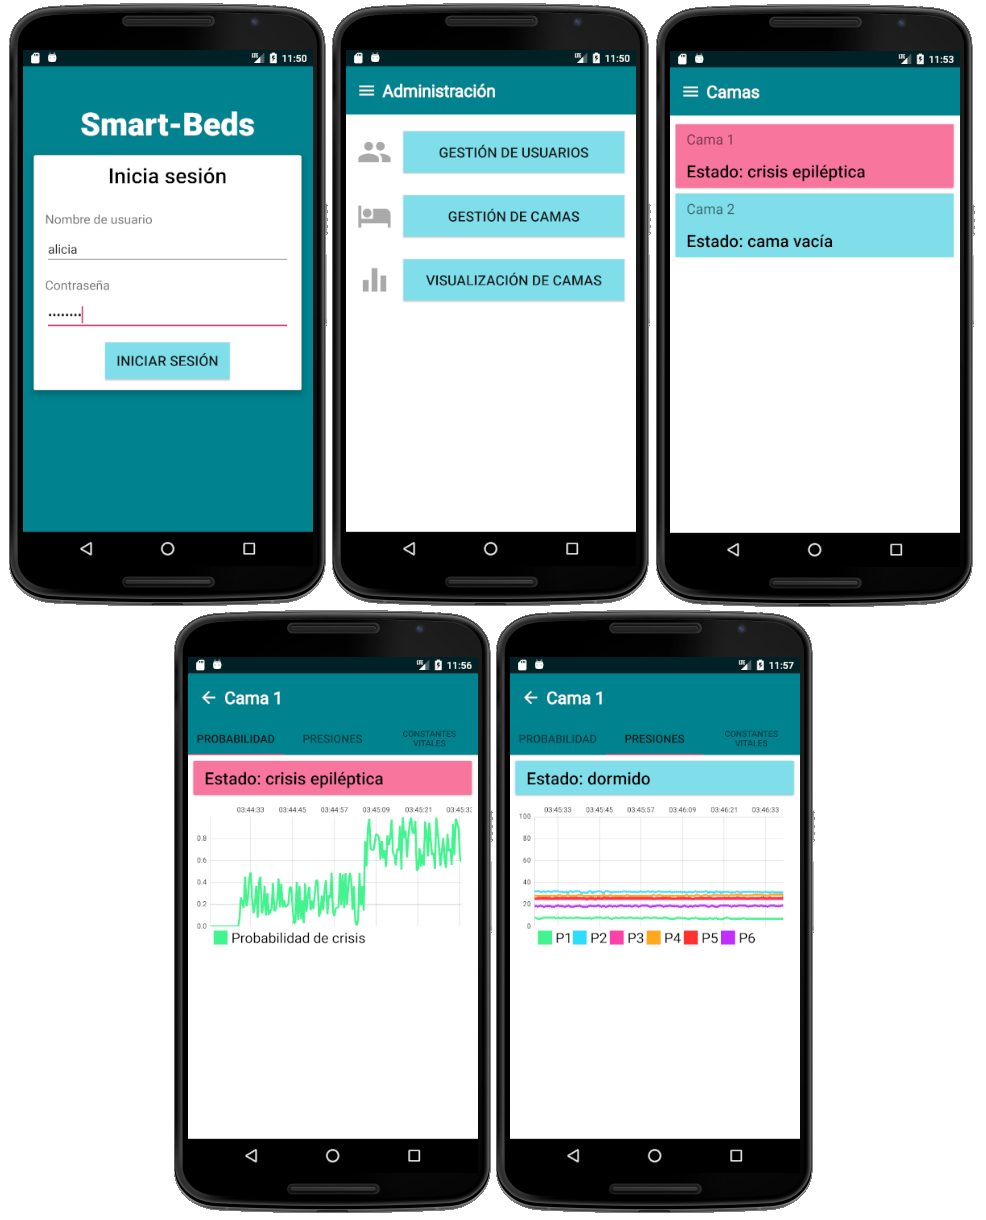
\includegraphics[width=0.75\textwidth]{../img/interfaces.png}
	\caption{Interfaces de usuario finales de las pantallas de: login, administración, visualización de camas y visualización de datos.}
	\label{fig:interfaces}
\end{figure}